\documentclass{article}
\usepackage[utf8]{inputenc} 
\usepackage{main}
%\graphicspath{ {./figs/} }

\title{ADASECANT: Robust Adaptive Secant Method for Stochastic Gradient}
%\iclrconference % Uncomment if submitted as conference paper instead of workshop
\author{
Caglar Gulcehre and Yoshua Bengio\\
Universit\'e de Montr\'eal \\
}
\begin{document}


\maketitle


\begin{abstract}
    Stochastic gradient algorithms have been the main focus of large-scale learning problems and 
    they led to impressive successes in machine learning. The convergence of SGD depends on the
    careful choice of learning rate and the amount of the noise in stochastic estimates of the gradients. 
    In this paper, we propose a new adaptive learning rate algorithm, which utilizes curvature information 
    for automatically tuning the learning rates. The information about the element-wise 
    curvature of the loss function is estimated from the local statistics of the stochastic first order
    gradients. We further propose a new variance reduction technique which automatically reduces the variance 
    of noise in the local gradient estimates to speed up the convergence. In our preliminary experiments with deep
    neural networks, we obtained better performance compared to the popular stochastic gradient algorithms.
\end{abstract}

\section{Introduction}

In  this paper we develop a stochastic gradient algorithm that reduces the burden of extensive 
hyper-parameter search for the optimization algorithm. The proposed algorithm exploits
a low variance estimator of curvature of the cost function and uses it to obtain an
automatically tuned adaptive learning rate for each parameter.

In the deep learning and numerical optimization, several papers suggest using a diagonal
approximation of the Hessian (second derivative matrix of the cost function with respect to
parameters), in order to estimate optimal learning rates for stochastic gradient descent over high dimensional
parameter spaces \citep{becker1988improving,schaul2012no,lecun1993automatic}. Among several proposals to estimate
the diagonal of Hessian efficiently, one option is to estimate it via the Gauss-Newton matrix \citep{lecun2012efficient} or 
by using finite differences \citep{schaul2013adaptive}. The diagonal estimations of the Hessian may however
be sensitive to noise due to the stochastic gradient.  \cite{schaul2012no} suggested a reliable 
way to estimate the local curvature in the stochastic setting. A fundamental advantage of using 
the diagonal estimation of the Hessian for deep learning problems is
that inverting the diagonal of the Hessian is a trivial and cheap operation. 
However note that the inverse of the diagonal Hessian is usually a bad approximation of the 
diagonal of inverse Hessian.

\cite{schaul2012no} kept track of the variance and average of the gradients in order to keep a 
reliable stochastic estimation of the diagonal Hessian matrix. In this paper, we follow a different approach: instead of using
a diagonal estimate of Hessian, we propose to estimate curvature along the direction of the
gradient and we apply a new variance reduction technique to compute this metric reliably. The root mean square
statistics and the variance of gradients are reduced adaptively by a very simple transformation. We keep
track of the estimation of curvature using a technique similar to that proposed by \cite{schaul2012no},
which uses the variability of the expected loss. Standard adaptive learning rate
algorithms only scale the gradients, but regular Newton-like second order methods, can perform
more complicate transformations, e.g. rotating the gradient vector. Newton and quasi-newton
methods can also be invariant to affine transformations in the parameter space. Our proposed
\textbf{Adasecant} algorithm is basically a stochastic rank-$1$ quasi-Newton method. But in comparison with other adaptive
learning algorithms, instead of just scaling the gradient of each parameter, Adasecant can also perform an affine
transformation on them.

\section{Directional Secant Approximation}
\label{sec:dir_sec_approx}

Directional Newton is a method proposed for solving equations with multiple variables
\citep{levin2002directional}.  The advantage of directional Newton method proposed in
\cite{levin2002directional}, compared to Newton's method is that, it does not require 
a matrix inversion and still maintains a quadratic rate of  convergence.

%The directional Newton update step proposed for is defined as follows:

%\begin{equation}
%\Delta^k = -\frac{\f(\TT^k)}{\nabla_{\TT} \f(\TT^k) \cdot \vd^k} \vd^k
%\end{equation}

In this paper, we develop a second-order directional Newton method for nonlinear optimization.
Step-size of update $\Delta^k$ for step $k$ can be written as if it were a diagonal matrix:

\begin{equation}
\label{eqn:dir_newton}
\Delta^k = - \diag(\vd^k)(\diag(\H \vd^k))^{-1} \nabla_{\TT} \f(\TT^k)
\end{equation}

where $\TT^k$ is the parameter vector at update $k$, $\f$ is the objective function and $\vd$ is a
unit vector of direction that the optimization algorithm should follow.

A reformulation of Equation \ref{eqn:dir_newton} for each diagonal element of the step-size would be:

\begin{equation}
\Delta_i^k = - \frac{\nabla_{\TT_i }\f(\TT^k)}{\sum_{j=1}^{N} \frac{\partial^2 \f(\TT^k)}{\partial\theta_i \partial\theta_j} d_j^k} d_i^k
\end{equation}

One potential option might be to use the R-op to compute the Hessian-vector product
\citep{schraudolph2002fast} for the update in Equation \ref{eqn:dir_newton}. Instead, 
writing $\vh_i=\nabla_{\TT}\frac{\partial \f(\TT^k)}{\partial \theta_i}$ for the $i^{th}$ row of the Hessian 
matrix $\H$ and using the {\em directional secant approximation},
\begin{equation}
t_i^k=\frac{d_i^k}{\vh^k_i\vd^k},
\end{equation}

The per-parameter learning rate is $t_{i}^k$ and $\vd^k$ is the unit vector along the direction that we want to estimate the
curvature at update $k$. We can rewrite the gradient scaling factor (learning rate) following \citet{an2005directional}:

\begin{equation}
\frac{d_i^k}{\vh_i^k \vd^k} \approx \frac{t_i^{k} d_i^k}{\nabla_{\TT_i} \f(\TT^k + \vt^{k} \vd^k) - \nabla_{\TT_i} f(\TT^k)}
\end{equation}

where $\nabla_{\TT_i} f(\TT^k)$ is the $i^{th}$ element of the gradient vector at update $k$.


To choose a good direction $\vd^k$ in the stochastic setting, we used the block-normalized
gradient vector for each weight matrix $\mW^i_k$ and bias vector $\vb^i_k$ where
$\TT=\left\{\mW^i_k, \vb^i_k\right\}_{i=1\cdots k}$ at each layer $i$ and update $k$,
   i.e. $\vd_{\mW^i_k}^k = \frac{\nabla_{\mW^i_k} \f(\TT)}{||\nabla_{\mW^i_k} \f(\TT)||_2}$ and 
$\vd_k = \left[ \vd_{\mW^0_k}^k \vd_{\vb^0_k}^k \cdots \vd_{\vb^l_k}^k\right]$ for a neural
network with $l$ layers. It is easy see that, for each stochastic gradient update the angle 
between the stochastic gradient and block-normalized gradient will still be less than $90$
degrees. Nevertheless block normalization of the gradients adds an additional noise to the stochastic 
gradient estimates. But in practice we did not observe any negative aspect of this.

The update step is defined as $\Delta_{i}^k = t_i^k d_i^k$. The per-parameter learning rate
$t_i^k$ can be estimated via a finite difference approximation,

\begin{equation}
t_i^k = \frac{\Delta_{i}^k}{\nabla_{\TT_i} \f(\TT^k + \Delta^k) - \nabla_{\TT_i} \f(\TT^k)},
\end{equation}
since, in the vicinity of the quadratic local minima,
\begin{align}
    \nabla_{\TT} \f(\TT^k + \Delta^k) - \nabla_{\TT} \f(\TT^k) \approx \H^{k} \Delta^k
\end{align}

We can therefore recover $\vt^k$ as
\begin{equation}
\vt^k = \diag(\Delta^k)(\diag(\H^{k} \Delta^k))^{-1}.
\end{equation}

The directional secant method, basically scales the gradient of each parameter with the curvature along the direction of the gradient vector 
and it is numerically stable.

%If $\vd^k = \H^{-1} \nabla_{\TT} \f(\TT) $, we would be recovering the exact Newton update rule.

\section{Variance Reduction for Robust Stochastic Gradient Descent}
\label{sec:var_reduction}

Variance reduction techniques for stochastic gradient estimators have been well-studied 
in the machine learning literature. Both \cite{wang2013variance} and \cite{johnson2013accelerating} proposed new
ways of dealing with this problem. In this paper, we propose a new variance reduction technique 
for stochastic gradient descent that just relies on the statistics related to the gradients. $\vg_i$
refers to the $i^{th}$ element of the gradient vector $\vg$  with respect to the parameters 
$\TT$ and $\E[\cdot]$, is for the expectation taken over minibatches and different trajectories of
parameters.

We propose to apply the following transformation to reduce the variance of the stochastic
gradients:

\begin{equation}
\label{sec:var_reduc}
\tilde{g_i}=\frac{g_i + \mathbf{\gamma_i}\E[g_i]}{1+\mathbf{\gamma_i}}
\end{equation}

The variance of the transformed stochastic gradient is:
%\begin{eqnarray}
\begin{align}
\E[||\tilde{g_i}-\E[g_i]||^2_2] &= \E[||\frac{g_i+\mathbf{\gamma_i}\E[g_i]}{1+\mathbf{\gamma_i}}-\E[g_i]||^2_2] \\
&= \frac{1}{(1+\mathbf{\gamma_i})^2}\E[||g_i-\E[g_i]||^2_2]
\end{align}
%\end{eqnarray}

This transformation will therefore reduce the variance of each stochastic gradient
$g_i$  by $(1+\mathbf{\gamma_i})^2$.

If the estimation of $\E[g_i]$ is unbiased than the bias of $\tilde{g_i}$ will be $0$ as well:
%\begin{eqnarray}
\begin{align}
\E[\tilde{g_i}]-\E[g_i] &= \E[\frac{g_i+\mathbf{\gamma_i}\E[g_i]}{1+\mathbf{\gamma_i}}]-\E[g_i] \\
 &= \E[\frac{g_i+\mathbf{\gamma_i}\E[g_i] - \E[g_i] - \mathbf{\gamma_i}\E[g_i]}{1+\mathbf{\gamma_i}}] \\
 &= 0
\end{align}
%\end{eqnarray}

However, in practice, our estimator of $\E[g_i]$ based on past values of $g_i$ 
will be biased because the parameters keep changing,
making averages of old values stale.
Nevertheless by changing $\gamma$, it is possible to control the bias-variance tradeoff. 
The optimal $\gamma$ for minimizing the bias of $\E[g_i]$ can be estimated 
by minimizing the following objective function:

\begin{equation}
\label{eqn:exp_gamma_cri}
\argmin_{\gamma_i} \E[||\tilde{g_i} - g_i^{\prime}||^2_2]
\end{equation}

where $\vg^{\prime}$ is the gradient we obtained in the next minibatch. 
We can find the optimal $\gamma$ in closed-form by finding the $\gamma$ that minimizes the
objective function in Equation $\ref{eqn:exp_gamma_cri}$. We assumed that $\gamma$ is strictly
positive real number. $\gamma_i$ is basically a correction term that reduces the variance and bias of the
stochastic gradients.

\begin{equation}
\label{eqn:exp_gamma_opt}
\frac{\partial \E[||\tilde{g_i} - g_i^{\prime}||^2_2]}{\partial \gamma_i}=0
\end{equation}

We satisfy Equation \ref{eqn:exp_gamma_opt} separately for each parameter,
yielding a separate $\gamma_i$ in $\mathbb{\gamma}$ for each gradient element $g_i$ in
$\vg$:

\begin{align}
\label{eqn:exp_gamma_opt2}
\frac{\partial \E[(\frac{g_i+\mathbf{\gamma_i}\E[g_i]}{1+\mathbf{\gamma_i}} - g_i^{\prime})^2]}{\partial \gamma_i}&=0 \\
\E[(\frac{g_i + \mathbf{\gamma_i}\E[g_i] }{1+\mathbf{\gamma_i}} - g_i^{\prime}) \frac{\partial (\frac{(g_i+\mathbf{\gamma_i}\E[g_i])}{1+\mathbf{\gamma_i}} - g_i^{\prime})}{\partial \gamma_i}]&=0 \\
\E[(\frac{g_i + \mathbf{\gamma_i} \E[g_i]}{1 + \mathbf{\gamma_i}} - g_i^{\prime}) 
(\frac{(g_i+\mathbf{\gamma_i}\E[g_i])-(1+\gamma_i)(\E[g_i])}{(1 + \mathbf{\gamma_i})^2})]&=0 \\
\E[(g_i + \mathbf{\gamma_i} \E[g_i] - (1+\gamma_i)g_i{\prime})(g_i - \E[g_i])]&=0 \\
\E[(g_i - g^{_i\prime} +\mathbf{\gamma_i}(\E[g_i]-g_i^{\prime}))(g_i - \E[g_i])]&=0 \\
\E[(g_i - g_i^{\prime})(g_i - \E[g_i])] = \gamma_i \E[(g_i-\E[g_i])(g_i^{\prime}-\E[g_i]))]&=0 \\
\gamma_i &= \frac{\E[(g_i - g_i^{\prime})(g_i - \E[g_i])]}{\E[(g_i-\E[g_i])(g^{_i\prime}-\E[g_i]))]}
\end{align}

As a result, in order to estimate $\gamma$ for each dimension, we should keep track of $\frac{\E[(g_i - g_i^{\prime})(g_i - \E[g_i])]}{\E[(g_i - \E[g_i])(g_i^{\prime}-\E[g_i]))]}$, 
during training.

\section{Adaptive Step-size in Stochastic Case}

In the stochastic gradient case, the step-size for directional secant can be computed by using an expectation over the minibatches:

\begin{equation}
\label{eqn:adapt_stepsize}
\E_k[t_{i}] = \E_k[\frac{\Delta_i^k}{\nabla_{\TT_i} \f(\TT^k +  \Delta^k) - \nabla_{\TT_i} \f(\TT^k)}]
\end{equation}

Considering that multiple passes are done over the dataset, the step size is computed as the expected value
of the directional secant over different minibatches and trajectories.

Computing the expectation in \ref{eqn:adapt_stepsize} was numerically very unstable in the stochastic
setting. Thus we decided to use a numerically more stable approximation of it. If we do a second order Taylor approximation of 
Equation \ref{eqn:adapt_stepsize} around $(\sqrt{\E_k[(\alpha_i^k)^2]}, \sqrt{\E_k[(\Delta_i^k)^2]})$, with $\alpha_i^k = \nabla_{\TT_i} \f(\TT^k + \Delta^k) - \nabla_{\TT_i} \f(\TT^k)$, 
and assume  $\sqrt{\E_k[(\alpha_i^k)^2]} \approx \E_k[\alpha_i^k]$ and $\sqrt{\E_k[(\Delta_i^k)^2]} \approx \E_k[\Delta_i^k]$ then we obtain:

\begin{align}
\label{eqn:step_size_stoc_der1}
& \E_k[t_{i}] \approx \frac{\sqrt{\E_k[(\Delta_i^k)^2]}}{\sqrt{\E_k[(\alpha_i^k)^2]}} -
\frac{\cov(\alpha_i^k,\Delta_i^k)}{\E_k[(\alpha_i^k)^2]} 
%& \E_k[t_{i}] \approx \frac{2\sqrt{\E_k[(\Delta_i^k)^2]}}{\sqrt{\E_k[(\alpha_i^k)^2]}} -
%\frac{\E_k[\alpha_i^k\Delta_i^k]}{\E_k[(\alpha_i^k)^2]} \label{eqn:step_size_stoc_der2}
\end{align}

Equation \ref{eqn:step_size_stoc_der1} should always be non-negative. In our experiments, 
we used a simpler approximation in Equation \ref{eqn:step_size_stoc2}, which in practice,
worked at least as well as the formulations in Equations \ref{eqn:step_size_stoc_der1}:

\begin{equation}
\label{eqn:step_size_stoc2}
\E_k[t_{i}] \approx \frac{\sqrt{\E_k[(\Delta_i^k)^2]}}{\sqrt{\E_k[(\alpha_i^k)^2]}} -
\frac{\E_k[\alpha_i^k\Delta_i^k]}{\E_k[(\alpha_i^k)^2]}
\end{equation}

%$\(E_k[\Delta_ii^k], E[\nabla_{\TT_i} \f(\theta^k + \Delta^k)_i - \nabla_{\TT_i} \f(\theta^k)]]$:

%\begin{equation}
%\ref{eqn:step_size_stoc1}
%E_k[t_{i}] \approx \frac{E_k[\Delta_ii^k]}{E_k[\nabla_{\TT_i} \f(\theta^k + \Delta^k)_i -
%    \nabla_{\TT_i} \f(\theta^k)]} - \frac{\cov(\Delta_i^k, \nabla_{\TT_i} \f(\TT^k + \Delta^k)_i -
%                                               \nabla_{\TT_i}\f(\TT^k))}{(E_k[\nabla_{\TT_i}
%        \f(\TT^k + \Delta^k) - \nabla_{\TT_i} \f(\TT^k)])^2} + \frac{\var(\nabla_{\TT_i}
%        \f(\TT^k + \Delta^k) - \nabla_{\TT_i} \f(\TT^k)) \Delta_i^k}{(E_k[\nabla_{\TT_i}
%        \f(\TT^k + \Delta^k) - \nabla_{\TT_i} \f(\TT^k)])^3}
%\end{equation}
%Or if we assume that $\alpha_i^k = \nabla_{\TT_i}
%        \f(\TT^k + \Delta^k) - \nabla_{\TT_i} \f(\TT^k)$ then,
%        $$E_k[t_{i}] = \frac{E_k[\Delta_i^k]}{E_k[\gamma_i^k]} - \frac{\cov(\Delta_i^k,\gamma^i_k)}{(E_k[\gamma_i^k])^2}
%        + \frac{\var(\gamma_i^k) \Delta_i^k}{(E_k[\gamma_i^k])^3}$$
%When $\var(\gamma_i^k) \rightarrow 0 $, we will have:

%\begin{equation}
%\ref{eqn:step_size_stoc2}
%E_k[t_{i}] = \frac{E_k[\Delta_i^k]}{E_k[\gamma_i^k]} + \frac{\E_k[(\Delta_i^k\gamma^i_k]}{(E_k[\gamma_i^k])^5}
%\end{equation}

%We kept the root-mean square statistics for the first term in Equation \ref{eqn:step_size_stoc2}:
%$\E_k[t_{i}] = \sqrt{\frac{\E_k[(\Delta_i^k)^2]}{\E_k[(\gamma_i^k)^2]}} -
%\frac{\cov(\Delta_i^k,\gamma^i_k)}{(\E_k[\gamma_i^k])^2}$$

\section{Algorithmic Details}

\subsection{Approximate Variability}
To compute the moving averages as also adopted by \cite{schaul2012no}, 
we used an algorithm to adaptively decide the time constant based on the step size being taken. 
As a result algorithm that we used will give larger weights to the updates that has large step-size 
and smaller weight to the updates that has smaller step-size.

By assuming that $\bar{\Delta}_i[k]\approx\E[\Delta_i]_k$, 
the moving average update rule for $\bar{\Delta}_i[k]$ can be written as,
\begin{align}
    \label{eqn:approx_var}
    & \bar{\Delta}_i^2[k] = (1~-~\tau_i^{-1}[k])\bar{\Delta}_i^2[k-1] + \tau_i^{-1}[k](t_i^k
                                                                                   \tilde{\vg}_i^k)
    \\
    & \bar{\Delta}_i[k] = \sqrt{\bar{\Delta}_i^2[k]}
\end{align}

This update rule effectively assigns different weight for each element in the gradient vector and for each different update.
At each update, a scalar multiplication is performed with $\tau_i^{-1}$ and it is adapted during the training by using the following equation:
\begin{equation}
    \label{eqn:approx_var_update}
    \tau_i[k] = (1~-~\frac{\E[\Delta_i]_{k-1}^2}{\E[(\Delta_i)^2]_{k-1}})\tau_i[k-1] + 1
\end{equation}

%To be able to estimate the $\E[(\gamma_i^k)^2]$ we have used the corrected gradients that are
%introduced in Section \ref{sec:var_reduction}.
\subsection{Outlier Gradient Detection}

We used an outlier detection algorithm which resets the time-constant when an outlier gradient 
is detected. Our algorithm is very similar to \cite{schaul2013adaptive}, but instead of
incrementing $\tau_i[t+1]$ when an outlier is detected, the time-constant is reset by reinitializing
it to $2.2$. Noting that when $\tau_i[t+1] \approx 2$, this approximately assigns same amount of
weight for the current and the average of previous observations.  This outlier detection mechanism helped learning to become more stable, 
because when an outlier gradient is detected, empirically it tends to cause $\tau_i$ to saturate 
to a large value as well.

\subsection{Variance Reduction}
The correction parameter $\gamma$ is adapted based on the observed gradients with the Equation given in Section
\ref{sec:var_reduction}. This enables us to perform a fine-grained level of variance reduction for each
parameter independently, by using the estimates of 
\[
  \gamma^k_i =\frac{\E[(g_i - g_i^{\prime})(g_i - \E[g_i])]_k}{\E[(g_i-\E[g_i])(g_i^{\prime}-\E[g_i]))]_k}.
\]
If we use the variance reduction technique covered in Section \ref{sec:var_reduction},
   asymptotically it is possible to recover the batch gradient descent. The noise in the stochastic
   gradient methods can have advantages both in terms of generalization and optimization. But the noise 
   also introduces an exploration and exploitation trade-off. It is possible to fine-tune this trade-off 
   by thresholding the values of $\gamma$. We upper bounded $\gamma$ with a maximum threshold value $\rho_i$. Such that, 
   thresholded $\gamma_i$ will be estimated by $\gamma_i^{\prime}=\text{minimum}(\rho_i, \gamma_i)$.

We block-wise normalized the gradients of each weight matrix and bias vectors in $\vg$ to compute the
$\tilde{\vg}$, for example the gradient $\vg_{\W^{(i)}}$ of weight matrix $\W^{(i)}$ is ensured to be
$\frac{\vg_{\W^{(i)}}}{||\vg_{\W^{(i)}}||_2^2}$ as described in Section \ref{sec:dir_sec_approx}. The block-normalization of 
$\vg$ makes the Adasecant to be scale-invariant, hence more robust to the scale of the inputs and the number of the layers of the network.
We also empirically observed that, it was easier to train very deep neural networks with block normalized gradient descent.

\section{Improving Convergence}
Classical convergence results for SGD are based on the conditions,
\[
  \sum_i (\eta^{(i)})^2 < \infty
\]
and 
\[
  \sum_i \eta^{(i)} = \infty,
\]
such that the learning rate $\eta^{(i)}$ should decrease \citep{robbins1951stochastic}. Due to the noise in the estimation of
adaptive step-sizes for Adasecant, the convergence is still not strictly guaranteed. To ensure convergence, 
we developed a new variant of Adagrad \citep{duchi2011adaptive}. We thresholded Adagrad, such that each Adagrad scaling factor 
is lower bounded by $1$. Assume  $a_i^k$ is the accumulated norm of all past gradients for $i^{th}$ parameter at update $k$:
\begin{equation}
a_i^k = \sqrt{\sum_{j=0}^k (g_i^j)^2}
\end{equation}
The $a_i^k$ is thresholded from below by simply using 
\begin{equation}
\rho_i^k = \text{maximum}(1, a_i^k), 
\end{equation}
to ensure that the algorithm
will eventually converge:

\begin{equation}
 \Delta_i^k = \frac{1}{\rho_i}\eta_i^k\tilde{\vg}_i^k
\end{equation}

In the initial stages of training, accumulated norm of the per-parameter gradients can be less than $1$. If the
accumulated per-parameter norm of a gradient is less than $1$, Adagrad will augment 
the learning-rate determined by Adasecant for that update, i.e.
$\frac{\eta_i^k}{\rho_i^k} > \eta_i^k$ where $\eta_i^k=\E_k[t_i^k]$ is the per-parameter learning rate determined
by Adasecant. This behavior tends to create unstabilities during the training
with Adasecant. Our modification of the Adagrad algorithm is to ensure that, it will
 reduce the learning rate determined by the Adasecant algorithm at each update, i.e. $\frac{\eta_i^k}{\rho_i^k} \le
 \eta_i^k$ and the learning rate will be bounded. In the beginning of training, parameters of a
 neural network can get $0$-valued gradients, e.g. in the existence of dropout and ReLU units. 
 However this phenomena can cause the per-parameter learning rate scaled by Adagrad to be
 unbounded. 

In Algorithm \ref{alg:adasecant}, we provide a simple pseudo-code of the Adasecant algorithm.

\begin{algorithm}[htb]
%\DontPrintSemicolon
\SetKwInOut{Input}{input}
\SetKwInOut{Output}{output}
\label{alg:adasecant}
\caption{Adasecant: minibatch-Adasecant for adaptive learning rates with variance reduction}

 \Repeat{stopping criterion is met}{
  draw $\popsize$ samples,
  compute the gradients $\vg^{(j)}$ where $\vg^{(j)} \in \R^{n}$ for each minibatch $j$,
  $\vg^{(j)}$ is computed as,~$\frac{1}{\popsize}\sum_{k=1}^{\popsize}\nabla_{\TT}^{(k)}\f(\TT)$ \\ 
  block-wise normalize gradients of each weight matrix and bias vector \\
  \For{\text{parameter} $i \in \{1, \ldots, n\}$}{
    compute the correction term by using, $\gamma^k_i =\frac{\E[(g_i - g_i^{\prime})(g_i - \E[g_i])]_k}{\E[(g_i-\E[g_i])(g_i^{\prime}-\E[g_i]))]_k}$ \\
  	compute corrected gradients $\tilde{g_i}=\frac{g_i+\mathbf{\gamma_i}\E[g_i]}{1+\mathbf{\gamma_i}}$ \\
  	\vspace{0.5em}
    \If{$|g_i^{(j)}- \E[g_i]| > 2 \sqrt{\E[(g_i)^2]-(\E[g_i])^2} \;\;\; \operatorname{or} \;\;\;
        \left|\alpha_i^{(j)} - \E[\alpha_i]\right| > 2 \sqrt{\E[(\alpha_i)^2] - (\E[\alpha_i])^2}$}
  	{\vspace{0.5em}
  	reset the memory size for outliers $\tau_i \leftarrow 2.2$}{}
  	\vspace{0.5em}
    update moving averages according to Equation \ref{eqn:approx_var} \\
\vspace{0.5em}
  estimate learning rate $\;\;\displaystyle\eta_i^{(j)} \leftarrow
      \frac{\sqrt{\E_k[(\Delta_i^{(k)})^2]}}{\sqrt{\E_k[(\alpha_i^k)^2]}} -
      \frac{\E_k[\alpha_i^k\Delta_i^k]}{\E_k[(\alpha_i^k)^2]}$\\
  \vspace{0.5em}
  update memory size as in Equation \ref{eqn:approx_var_update}\\
 \vspace{0.5em}
 update parameter $\;\; \theta_i^j \leftarrow \theta_i^{j-1} - \eta_i^{(j)}\cdot \tilde{g}_i^{(j)}$\\
 }
 }

\end{algorithm}


\section{Experiments}
We have performed our experiments on MNIST with Maxout Networks \citep{goodfellow2013maxout}.

We have compared our algorithm with other popular stochastic gradient learning algorithms have been tested as well,
Adagrad, Rmsprop \citep{graves2013generating}, Adadelta \citep{zeiler2012adadelta} and SGD+momentum (linearly decaying learning rate). 
Results are summarized in Figure~\ref{fig:depthexp} and show that Adasecant converges
as fast or faster than other techniques, including the use of hand-tuned global learning rate and momentum for SGD,
RMSprop, and Adagrad.

\begin{figure}[htbp]
\centering
\subfigure[$2$ layer Maxout Network]{
\label{fig:depthexpa}
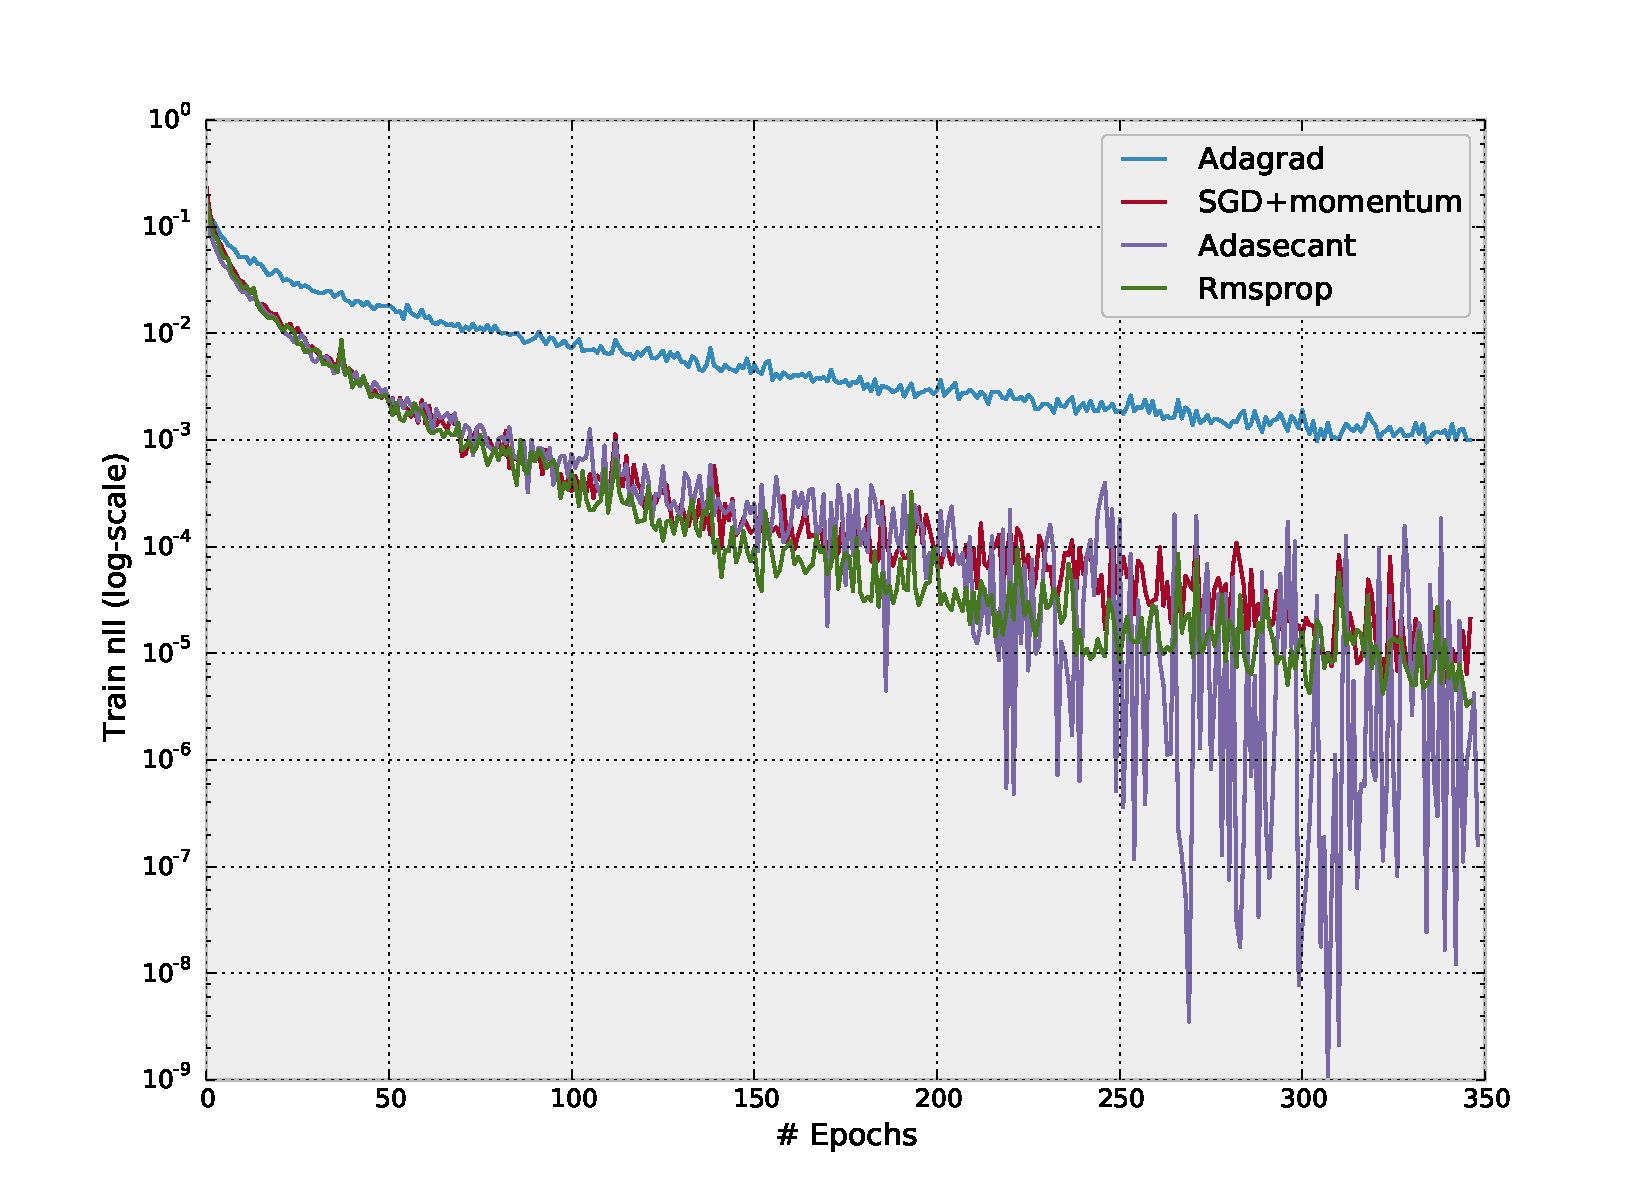
\includegraphics[width=7cm]{adasecant_cmps_mnist_maxout.pdf}
}
\subfigure[$16$ layer Maxout Network]{
\label{fig:depthexpb}
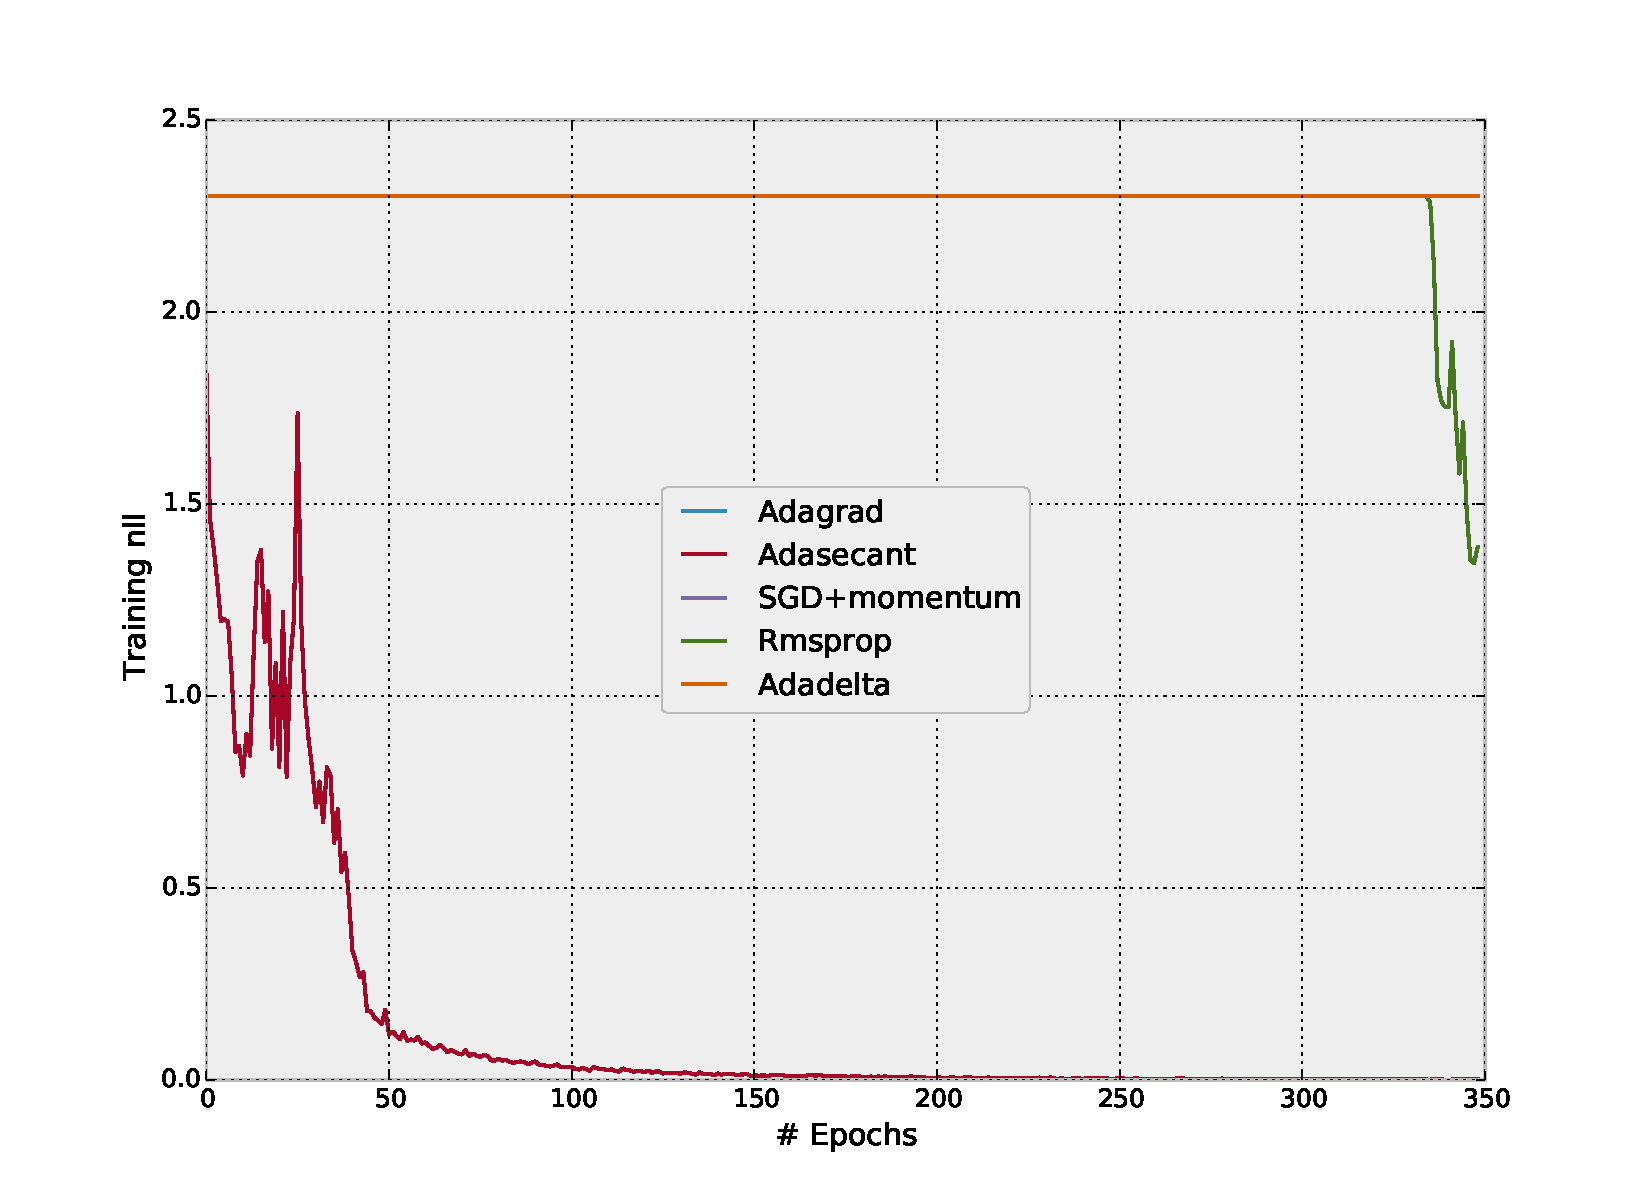
\includegraphics[width=7cm]{radaprop_train_log_scale_nll.pdf}
}
\caption{Comparison of different stochastic gradient algorithms on MNIST with Maxout Networks.
    Both a) and b) are trained with dropout and maximum column norm constraint regularization on
    the weights. Networks are initialized with weights sampled from a Gaussian distribution with
    $0$ mean and standard deviation of $0.05$. In both experiments, the proposed algorithm,
    Adasecant, seems to be converging faster and arrives to a better minima in training set. We trained both
    networks for $350$ epochs over the training set.}
\label{fig:depthexp}
\end{figure}

\section{Conclusion}
We provided a new stochastic gradient algorithm with adaptive learning rates
that is fairly insensitive to the tuning of the hyper-parameters and doesn't require tuning of learning
rates. Furthermore, the variance reduction technique we provided for SGD improves the
convergence in the settings where stochastic gradients have high variance. We provided a set of preliminary
results with deep neural networks. According to our preliminary experiments, we were able to obtain better
training performance compared to other well-tuned popular stochastic gradient algorithms. As a future
work, we should do a more comprehensive analysis, which will help us to better understand
the algorithm both analytically and empirically.

\vspace*{-1mm}
\subsubsection*{Acknowledgments}
\vspace*{-1mm}

We thank the developers of Theano \citep{Bastien-2012} and Pylearn2 \citep{pylearn2_arxiv_2013} and the computational resources
provided by Compute Canada and Calcul Qu\'ebec. This work has been partially supported by NSERC,
CIFAR, and Canada Research Chairs, Project TIN2013-41751, grant 2014-SGR-221. We would 
like to thank Tom Schaul for the valuable discussions. We also thank Kyunghyun Cho and Orhan Firat
for proof-reading and giving feedbacks on the paper.

{\small
\bibliography{myref}
\bibliographystyle{natbib}}

\appendix
\section{Appendix}
\subsection{Experimental Details}
In our experiments with Adasecant algorithm, adaptive momentum term $\gamma_i^k$ was clipped at
$1.8$. In $2$-layer Maxout network experiments for SGD-momentum experiments, we used the best hyper-parameters reported 
by \cite{goodfellow2013maxout}, for Rmsprop and Adagrad, we crossvalidated learning rate for $15$ different learning rates 
sampled uniformly from the log-space. We crossvalidated $30$ different pairs of momentum and learning rate for SGD+momentum,
for Rmsprop and Adagrad, we crossvalidated $15$ different learning rates sampled them from log-space uniformly
 for deep maxout experiments.

\end{document}
